\documentclass[a4paper, 12pt]{article}
\usepackage[a4paper,top=1.5cm, bottom=1.5cm, left=1cm, right=1cm]{geometry}
\usepackage[utf8]{inputenc}
\usepackage{mathtext}
\usepackage{amsmath}
\usepackage{amsfonts}
\usepackage[english, russian]{babel}
\usepackage{indentfirst}
\usepackage{longtable}
\usepackage{graphicx}
\graphicspath{{pictures/}}
\DeclareGraphicsExtensions{.pdf,.png,.jpg}
\usepackage{natbib}
\usepackage{mathrsfs}
%\usepackage[europeanresistors, americaninductors]{circuitikz}

\title{Лабораторная работа 1.3.2 Определение модуля кручения}
\author{Михаил Колтаков}
\date{29 октября 2020 г.}

\begin{document}
	\maketitle
	\section*{Цель работы}
		Измерение углов закручивания в зависимости от приложенного момента сил, расчёт модулей кручения и сдвига при статическом закручивании стержня, определение тех же модулей для проволоки по измерениям периодов крутильных колебаний подвешенного на ней маятника(динамическим методом)
	\section*{Оборудование}
		В первой части: исследуемый стержень, отсчётная туба со шкалой, рулетка, микрометр, набор грузов;
		во второй части: проволока из исследуемого материала, грузы, секундомер, микрометр, линейка, рулетка.
	\section*{Теория к работе}
		При закручивании цилиндрических стержней круглого сечения распределение деформаций одинаково по длине стержня только вдали от мест, где прикладываются закручивающие моменты. Для этих областей можно считать, что каждое поперечное сечение поворачивается как жёсткое, то есть частички материала не сходят с радиальных линий, где они находились вначале, и все эти радиальные лини поворачиваются на один и тот же угол. Напряжённое состояние, которое при этом возникает называется чистым кручением.
		
		При рассмотрении закручиваемого цилиндра длины l можно заметить, что любая прямая вертикальная линия, проведённая до закручивания превращается в спираль. Сечения на расстоянии l повёрнуты на угол $\Delta \varphi $
		
		Рассмотрев небольшие кусочки цилиндра, можно вывести соотношение
		$$ \tau = Gr \frac{d \varphi}{dl}$$
		
		$\tau$ - касательное напряжение
		
		$G$ - модуль сдвига
		
		Суммарный момент сил, действующий на всём поперечном сечении цилиндра радиуса $R$, создаваемый этими напряжениями, можно выразить как
		$$M=\pi G \frac{R^4}{2} \frac{d \varphi}{dl} $$
		Этот момент не меняется по длине цилиндра, значит, для поперечного сечения, находящегося на расстоянии l можно связать момент сил и угол его поворота.
		$$M = \frac{\pi R^4 G}{2l} \varphi = f \varphi$$
		Величина $f$ называется модулем кручения.
	\section*{Ход работы}
		\subsection*{I. Определение модуля кручения статическим методом}
				Эту часть работы будем проводить на установке, схематично изображённой ниже. Она состоит из вертикально расположенного стержня С, верхний конец которого прочно закреплён на стойке, а нижний соединён с диском Д. Момент $M$, закручивающий стержень создают две навитые на диск и перекинутые через блоки Б нити, к концам которых подвешиваются одинаковые грузы Г. Диск снабжён зеркальцем З. Для того, чтобы узнать угол поворота диска, нужно направить зрительную трубу на зеркальце и сделать так, чтобы в неё была чётко видна шкала, укреплённая на том же штативе, что и трубка. По изменению положения шкалы можно определить угол закручивания $\varphi$.
				
				\begin{figure}[h]
					\center{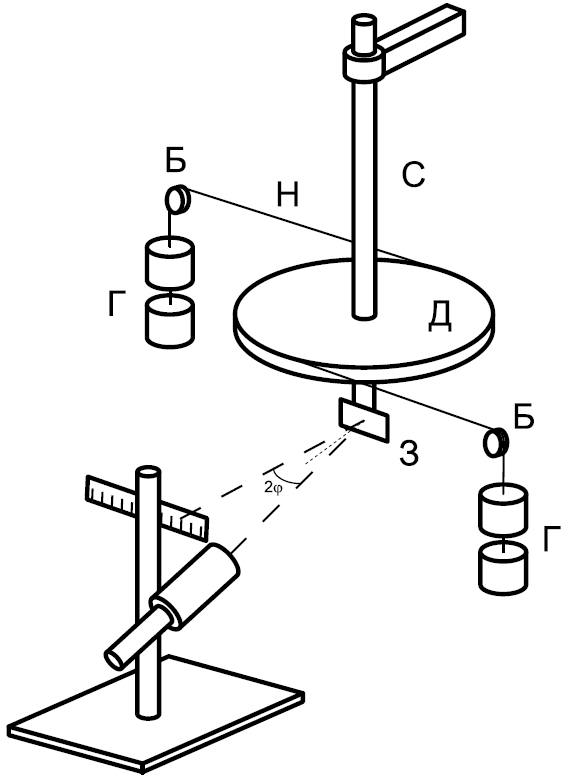
\includegraphics{picture1}}
				\end{figure}
				
				1. Установим зрительную трубку так, чтобы в неё чётко была видна шкала. Измерим расстояние от зеркальца до шкалы $l \approx 131,5 \pm 1 см$. Диаметр диска $d_д \approx 107,3 \pm 0,1 мм$, диаметр стержня $d_с \approx 5,34 \pm 0,01 мм $.
				
				2. Построим зависимость $\varphi(M)$, проводя серии измерений увеличивая и уменьшая массы грузов на нитях. Угол поворота можно определить по формуле $\varphi = arctg \frac{\Delta l}{2l}$, где $\Delta l$ - смещение шкалы, видимой в зрительной трубке. Результаты измерений занесём в таблицу.
				\begin{longtable}[H]{|c|c|c|c|}
					\hline
					Серия & $\Delta l$, см & M, $Н \cdot м$ & $\varphi$, ° \\
					\hline
					& 6,0 & 0,10 & 1,3 \\
					1 & 6,8 & 0,11 & 1,5 \\
					& 16,0 & 0,21 & 3,5 \\
					& 22,5 & 0,32 & 4,9 \\
					\hline
					& 6,3 & 0,10 & 1,4 \\
					2 & 7,7 & 0,11 & 1,7 \\
					& 16,1 & 0,21 & 3,5 \\
					& 23,6 & 0,32 & 5,1 \\
					\hline
					& 4,7 & 0,10 & 1,3 \\
					3 & 6,2 & 0,11 & 1,4 \\
					& 14,7 & 0,21 & 3,2 \\
					& 21,0 & 0,32 & 4,6 \\
					\hline
					& 4,5 & 0,10 & 1,3 \\
					4 & 6,2 & 0,11 & 1,4 \\
					& 14,7 & 0,21 & 3,2 \\
					& 21,4 & 0,32 & 4,6 \\
					\hline
					& 6,6 & 0,10 & 1,5 \\
					5 & 7,3 & 0,11 & 1,6 \\
					& 14,3 & 0,21 & 3,1 \\
					& 21,5 & 0,32 & 4,7 \\
					\hline
					& 5,8 & 0,10 & 1,3 \\
					6 & 8,0 & 0,11 & 1,8 \\
					& 15,7 & 0,21 & 3,4 \\
					& 22,7 & 0,32 & 4,9 \\
					\hline
				\end{longtable}
			С помощью МНК найдём $f \approx 3,8 \pm 0,1$ $\frac{Н \cdot м}{рад}$ и построим график по средним значениям.
			\begin{figure}[h]
				\center{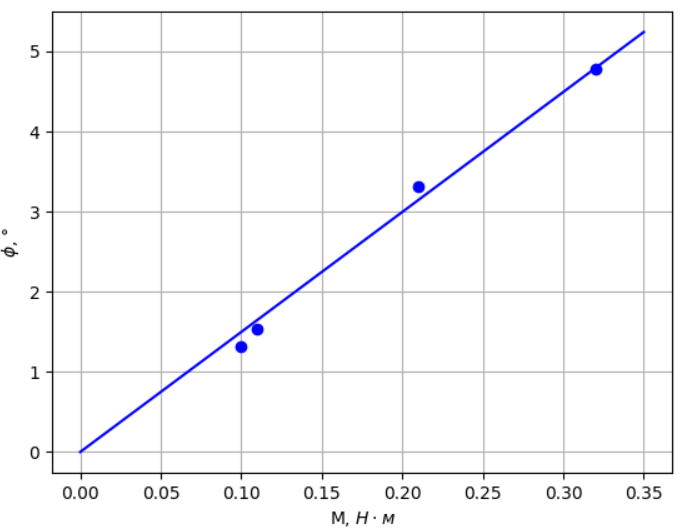
\includegraphics[scale=0.62]{graph1}}
			\end{figure}
			
			Модуль сдвига $G$ при этом получается равен $\frac{2lf}{\pi R^4} \approx 82,8 \pm 0,3 ГПа$
		\subsection*{II. Определение модуля кручения динамическим методом}
			Экспериментальная установка, использующаяся на данном этапе работы состоит из длинной висячей проволоки П, к нижнему её концу прикреплён горизонтальный стержень С, на котором симметрично закреплены грузики Г.
			
			\begin{figure}[h]
				\center{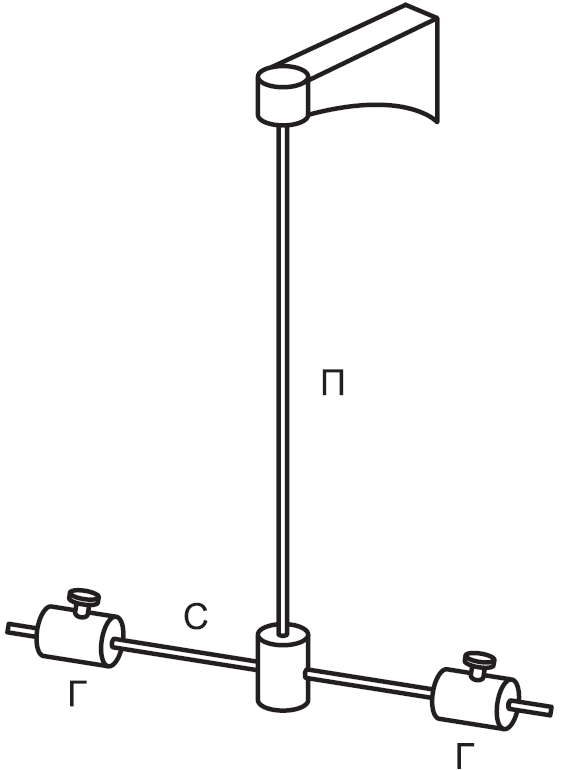
\includegraphics[scale=0.62]{picture2}}
			\end{figure}
			
			Период колебаний можно рассчитать по формуле
			$$T^2=\frac{(2 \pi)^2}{f} I_0 + \frac{(2 \pi)^2}{f} 2m \cdot l^2$$, где $I_0$ - момент инерции системы без грузов, $l$ - длина проволоки, $T$ - период колебаний при заданной длине $l$, а $m$ - масса одного груза.
					
			Построим график $T^2(l^2)$, тогда угловой коэффициент будет равен $k=\frac{(2 \pi)^2}{f} 2m$, отсюда $f=\frac{(2 \pi)^2}{k} 2m$
			
			\begin{figure}[h]
				\center{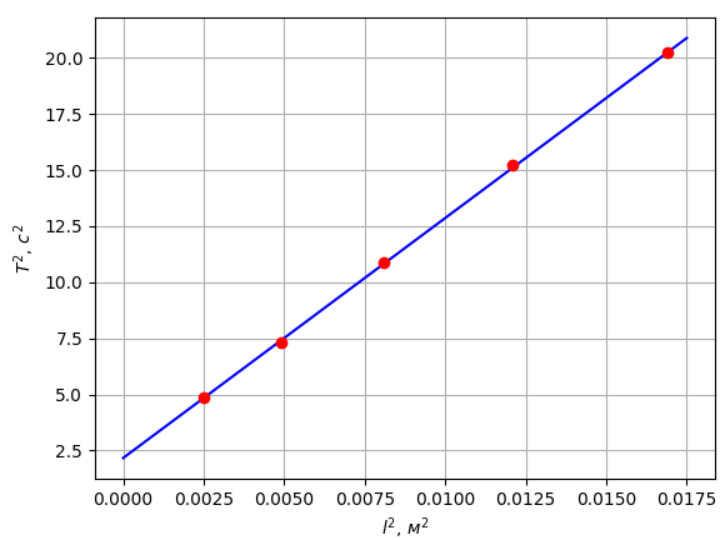
\includegraphics[scale=0.62]{graph2}}
			\end{figure}
			
			$k \approx 1070 \frac{с^2}{м^2}$, $f \approx \frac{(2 \pi)^2}{1070} 2 \cdot 0,376 \approx 0,03$ $\frac{Н \cdot м}{рад}$  при длине проволоки 170 см и её диаметре 1,55 мм. Тогда $G \approx 83,2 \pm 0,2 ГПа$.
	\section*{Вывод}
		Мы вычислили модули кручения двумя разными способами и на их основе определили модули сдвига материала. Полученные значения лежат очень близко друг к другу, так что эксперимент можно считать удачным.
\end{document}
